\section{Exercising data subject rights with DPV}
\label{sec:rights_exercising}

This Section describes the usage of vocabulary-based patterns to describe rights exercising metadata.
Such patterns can be used by entities dealing with the handling of personal data to maintain consistent records of data subject rights exercising activities, aligned with GDPR requirements.
In a decentralised data system environment, these rights must also be fulfilled by data controllers, while notices and records can be kept by data subjects in their personal datastores for transparency and accountability.

\subsection{Requirements to express rights-related activities}
\label{sec:rights_concepts}

This Section outlines the motivation and identified requirements for the expression of information related to the exercising of data subject rights.
This work was developed (and is already integrated) within the context of the DPVCG and was started with the main objectives of indicating (i) what rights exist (in particular within the framework of the GDPR), (ii) where such rights can be exercised, and (iii) what information needs to be recorded and maintained when a concrete instance of a right is being/was exercised.

As previously mentioned in Section~\ref{sec:def_gdpr} and represented in Figure~\ref{fig:gdpr_information_flows}, the focus of this Thesis is on the representation of information related to legislation on data protection in the European Union, in particular regarding the GDPR and related data subject rights, listed on Chapter III.
Moreover, in Section~\ref{sec:sota_vocabularies_criteria}, and in particular in Table~\ref{tab:GDPR_privacy_terms}, the privacy terms that need to be represented for such rights to be exercised by data subjects and fulfilled by data controllers.

From this analysis, a set of high-level concepts was proposed and adopted by the DPVCG (general concepts on Rights are modelled in the main DPV specification at \url{https://w3id.org/dpv#vocab-rights} and GDPR-specific ones in the DPV-GDPR extension at \url{https://w3id.org/dpv/dpv-gdpr#vocab-rights}).
Figure~\ref{fig:rights_dpv}, adapted from \cite{pandit_primer_2022}, provides an overview of these concepts.

\begin{figure}[ht]
    \centering
    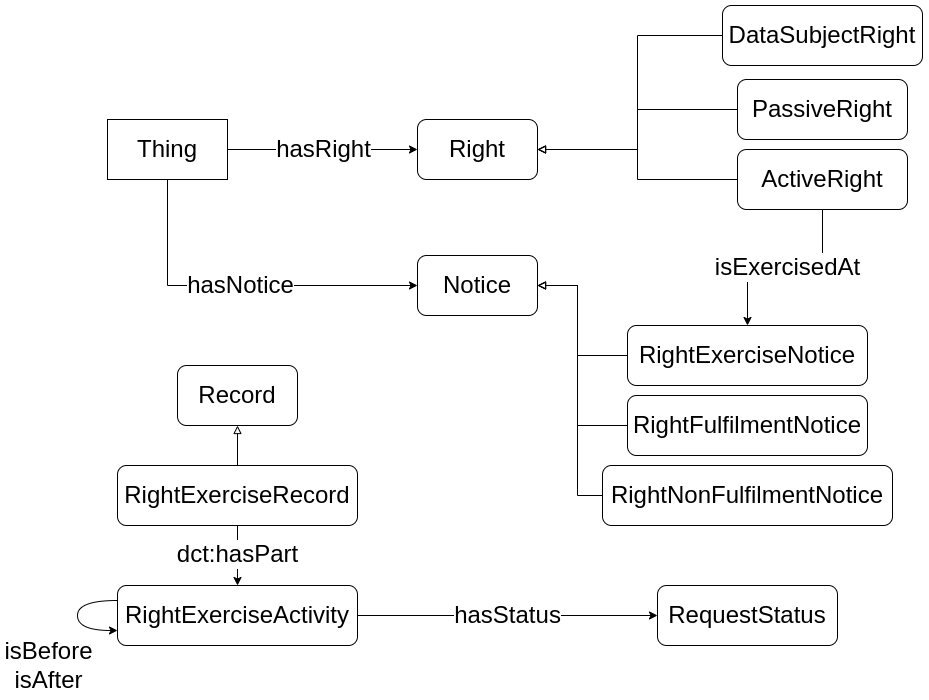
\includegraphics[width=\linewidth]{figures/chapter-4/DPV-rights.png}
    \caption{Core concepts of DPV's rights taxonomy, adapted from \cite{pandit_primer_2022} .}
    \label{fig:rights_dpv}
\end{figure}

Thus, beyond modelling concepts for applicable \texttt{Right}s and \texttt{DataSubjectRight}s (applicable only to data subjects), to indicate the association of concepts with a particular right, the \texttt{hasRight} property is also modelled in DPV.
Additionally, to make a distinction between actionable and non-actionable rights, the \texttt{ActiveRight} and \texttt{PassiveRight} concepts were created to distinguish between rights that require an action to be taken for them to be exercised and rights that don't require any action and are always applicable.% add examples of active/passive rights
To fulfil the second objective of establishing where such active rights can be exercised, DPV's \texttt{isExercisedAt} property should be used to connect the right with the \texttt{RightExerciseNotice}.
This notice provides contextual information regarding how to exercise a right.
Specialised notice concepts for rights that can be fulfilled and those that cannot are modelled as \texttt{RightFulfilmentNotice} and \texttt{RightNonFulfilmentNotice}, respectively.

Moreover, to represent concrete records of rights being exercised, the \texttt{RightExerciseRecord} concept, specified as a subclass of DPV's \texttt{Record}, can be used to associate a particular request, or even distinct requests from the same data subject, with corresponding rights exercising activities, modelled as \texttt{RightExerciseActivity}, using the DCMI Metadata Terms \texttt{hasPart} property.
Such activity instances should include metadata, e.g., timestamps, duration, or involved entities, to track the provenance of a particular right exercising process, from the request itself to its acknowledgement by the data controller and to the fulfilment or non-fulfilment of the right.
Additionally, to track the status of rights exercising activities, a set of request statuses are modelled in DPV, including \texttt{RequestAccepted} for a request being accepted towards fulfilment, \texttt{RequestRejected} for a request being rejected towards non-fulfilment or \texttt{RequestRequiresAction} for a request requiring an action to be performed from another party, and the \texttt{isBefore} and \texttt{isAfter} concepts can be used to specify that a specific activity occurs before or after another activity.

While this modelling was inspired by the GDPR, the concepts are described in a jurisdiction-agnostic manner so that they can be used to tackle data protection regulations in different jurisdictions.
For GDPR-specific rights, the \texttt{DataSubjectRight} concept is extended in DPV-GDPR with the data subject rights described in GDPR's Articles 13 to 22, as well as the rights to withdraw consent and to lodge a complaint with a supervisory authority, described in Articles 7.3 and 77.
A collection of justifications for non-fulfilment of data subject rights, extracted from the GDPR and illustrated in Table~\ref{tab:justifications}, was also modelled (as subclasses of a high-level \texttt{RightNonFulfilmentJustification} concept) and is already approved to be integrated into DPV-GDPR's outputs.
Moreover, notices for direct and indirect data collection, to fulfil the information requirements in Articles 13 and 14, for Subject Access Requests (SARs), described in Article 15, and for notifying recipients, necessary to fulfil the communication requirements of Articles 16, 17 and 18, are provided as GDPR-specific subclasses of \texttt{RightFulfilmentNotice}s.

% rights non-fulfilment justifications issue: https://github.com/w3c/dpv/issues/63 & meeting minutes:https://www.w3.org/2022/10/19-dpvcg-minutes.html
\begin{table}
    \centering
    \caption{Justifications for non-fulfilment of GDPR's data subject rights.}
    \label{tab:justifications}
    \resizebox{\textwidth}{!}{%
    \begin{tabular}{c|p{8.5cm}|c}
        \textbf{Term} & \textbf{Label} & \multicolumn{1}{c}{\begin{tabular}[c]{@{}c@{}} \textbf{GDPR} \\ \textbf{Article(s)} \end{tabular}} \\
        \hline\hline
        \texttt{RightNonFulfilmentJustification} & Justifications for non-fulfilment of a right & \\
        \hline\hline
        \texttt{IdentityVerificationFailure} & Identity of the data subject could not be verified & 12.2 \\
         \hline
        \texttt{ExcessiveRequest} & Request was excessive in scope & 12.5 \\
         \hline\hline
        \texttt{DataSubjectAlreadyInformed} & \multicolumn{1}{l|}{\begin{tabular}[l]{@{}l@{}} Data subject already has been provided with this\\ information \end{tabular}} & 13.4, 14.5(a) \\
         \hline
        \texttt{ImpairProcessing} & Fulfilment would cause impairment to processing & 14.5(b) \\
        \hline     
        \texttt{ExtraordinaryEffort} & Fulfilment would require extraordinary effort & 14.5(b), 19 \\
         \hline
        \texttt{RenderImpossible} & Fulfilment would be impossible & 14.5(b), 19 \\
         \hline
        \texttt{AlreadyDisclosed} & \multicolumn{1}{l|}{\begin{tabular}[l]{@{}l@{}} Information to be provided is already disclosed in\\ a Member State or Union law \end{tabular}} & 14.5(c) \\
         \hline
        \texttt{ConfidentialityObligation} & \multicolumn{1}{l|}{\begin{tabular}[l]{@{}l@{}} Fulfilment would compromise existing confidentiality\\ obligations \end{tabular}} & 14.5(d) \\
         \hline\hline
        \texttt{SafeguardPublicInterest} & \multicolumn{1}{l|}{\begin{tabular}[l]{@{}l@{}} Fulfilment would interfere with necessary tasks\\ carried out for public interest \end{tabular}} & 21.6 \\
         \hline\hline
        \texttt{FulfilContract} & \multicolumn{1}{l|}{\begin{tabular}[l]{@{}l@{}} Task is necessary for entering into, or performance\\ of a contract between data subject and controller \end{tabular}} & 22.2(a) \\
         \hline
        \texttt{AuthorisedByMemberStateLaw} & Task is authorised by Member State or Union Law & 22.2(b) \\
        \hline\hline
        \texttt{ConfidentialityBreach} & Fulfilment would result in a confidentiality breach & 23.1 \\
         \hline
        \texttt{SafeguardThirdPartyRights} & \multicolumn{1}{l|}{\begin{tabular}[l]{@{}l@{}} Fulfilment would adversely affect the rights of other\\ data subjects or third parties \end{tabular}} & 23.1 \\
         \hline
        \texttt{ConfidentialityOfOpinion} & \multicolumn{1}{l|}{\begin{tabular}[l]{@{}l@{}} Fulfilment would compromise existing confidentiality\\ regarding the expression of opinion \end{tabular}} & 23.1 \\
         \hline
        \texttt{PreventInvestigation} & \multicolumn{1}{l|}{\begin{tabular}[l]{@{}l@{}} Fulfilment would compromise or hinder an existing\\ investigation \end{tabular}} & 23.1 \\
         \hline
        \texttt{ImpairArchivingPurposes} & \multicolumn{1}{l|}{\begin{tabular}[l]{@{}l@{}} Fulfilment would compromise or hinder archiving\\ purposes \end{tabular}} & 23.1 \\
         \hline
        \texttt{ExemptFromDisclosure} & Information is legally exempt from disclosure & 23.1 \\
         \hline
        \texttt{SafeguardNationalSecurity} & \multicolumn{1}{l|}{\begin{tabular}[l]{@{}l@{}} Fulfilment would pose a threat to safeguard\\ national security \end{tabular}} & 23.1 \\
         \hline
        \texttt{SafeguardDefence} & Fulfilment would pose a threat to safeguard defence & 23.1 \\
         \hline
        \texttt{SafeguardPublicSecurity} & \multicolumn{1}{l|}{\begin{tabular}[l]{@{}l@{}} Fulfilment would pose a threat to safeguard public\\ security \end{tabular}} & 23.1 \\
         \hline
        \texttt{SafeguardJudicialIndependence} & \multicolumn{1}{l|}{\begin{tabular}[l]{@{}l@{}} Fulfilment would pose a threat to safeguard judicial\\ independence or proceedings \end{tabular}} & 23.1 \\
    \end{tabular}}
\end{table}
% Information is legally exempt from disclosure	- Documents that have personal data of the data subject exempt from disclosure in court proceedings apply in relation to a Subject Access Request, this applies to both legal advice and litigation privilege

An overview of the aforementioned requirements and the intended purpose for modelling these concepts is presented in the ORSD illustrated in Table~\ref{tab:rights_ORSD}.

\begin{table}[htbp]
\centering
\caption{ORSD of the proposed model to express rights-related activities.}
\label{tab:rights_ORSD}
\scriptsize
\begin{tabular}{| l | l | l | l  | l | l | l |l| }
\hline
\multicolumn{8}{|c|}{\cellcolor[HTML]{A0A0A0}\textbf{Vocabulary-based patterns for rights exercising activities}} \\ \hline
\multicolumn{8}{|c|}{\cellcolor[HTML]{EFEFEF}\textbf{1. Purpose}} \\ \hline
\multicolumn{8}{| p{12.0cm} |}{The purpose of this model is the expression of rights-related activities, in particular focusing on data subject rights, such as the ones described in GDPR's Chapter III.} \\ \hline
\multicolumn{8}{|c|}{\cellcolor[HTML]{EFEFEF}\textbf{2. Scope}} \\ \hline
\multicolumn{8}{| p{12.0cm} |}{The scope of this model is limited to the expression of information related to the various steps of exercising data subject rights. In particular, the introduced concepts serve one of these purposes: (i) indicate what rights exist, (ii) express where such rights can be exercised, and (iii) record information related to concrete instances of rights that are being or were exercised. } \\ \hline
\multicolumn{8}{|c|}{\cellcolor[HTML]{EFEFEF}\textbf{3. Implementation Language}} \\ \hline
\multicolumn{8}{| p{12.0cm} |}{RDF, RDFS} \\ \hline
\multicolumn{8}{|c|}{\cellcolor[HTML]{EFEFEF}\textbf{4. Intended End-Users}} \\ \hline
\multicolumn{8}{| p{12.0cm} |}{Developers of Web services and applications, including decentralised storage solutions, that handle personal data.} \\ \hline
\multicolumn{8}{|c|}{\cellcolor[HTML]{EFEFEF}\textbf{5. Intended Uses}} \\ \hline
\multicolumn{8}{| p{12.0cm} |}{
Use 1. Declaration of the existence of data subject rights when the usage and collection of personal data is performed by Web services providers and developers, including information on where they can be exercised. \newline
Use 2. Patterns for data subject rights that can be fulfilled. \newline
Use 3. Patterns for data subject rights that cannot be fulfilled, including justifications for non-fulfilment. \newline
Use 4. Fulfilment of data subject rights requests from specific data protection legislation, such as the GDPR.
 } \\ \hline
\multicolumn{8}{|c|}{\cellcolor[HTML]{EFEFEF}\textbf{6. Ontology Requirements}} \\ \hline
\multicolumn{8}{|c|}{\cellcolor[HTML]{EFEFEF}\textbf{a. Non-Functional Requirements}}    \\ \hline
\multicolumn{8}{| p{12.0cm} |}{
NFR 1. The concepts are either published online within DPVCG's outputs, following W3C's specification format, or are under discussion for being adopted by the same CG. } \\ \hline
\multicolumn{8}{|c|}{\cellcolor[HTML]{EFEFEF}\textbf{b. Functional  Requirements: Groups of Competency Questions}}  \\ \hline
\multicolumn{5}{|c|}{\cellcolor[HTML]{EFEFEF}CQG1. Related to data subject rights} & \multicolumn{3}{|c|}{\cellcolor[HTML]{EFEFEF}CQG2. Related to GDPR} \\ \hline
\multicolumn{5}{ | m{7cm} |}{
CQ1. What rights are applicable in a given context? \newline
CQ2. Where can the right be exercised? \newline
CQ3. How can the right be exercised? \newline
CQ4. What data is necessary to implement the right? \newline 
CQ5. Which entity implements the right? \newline 
CQ6. Which entity exercised the right? \newline 
CQ7. When is the exercising activity occurring? \newline 
CQ8. What is the status of the right request? } & 
\multicolumn{3}{ m{5cm} |}{
CQ9. Which data subject rights are applicable according to the legal basis used by the data controller? \newline
CQ10. Which provenance metadata must controllers provide when replying to data subject rights requests? \newline 
CQ11. Which justification can be provided to not fulfil a request?
}\\ \hline
\end{tabular}
\vspace{-0.1in}
\end{table}

\subsection{Vocabulary-based patterns for rights exercising activities}
\label{sec:rights_patterns}

This Section outlines the usage of DPV for the expression of rights exercising activities, specifically related to the data subject rights described in GDPR's Chapter III.
Accordingly, the \textit{``controller shall take appropriate measures to provide any information referred to in Articles 13 and 14 and any communication under Articles 15 to 22 [...] to the data subject in a concise, transparent, intelligible and easily accessible form''} and if \textit{``the data subject makes the request by electronic form means, the information shall be provided by electronic means where possible, unless otherwise requested by the data subject''} \citeyearpar{noauthor_regulation_2016}.
Consequently, in this Thesis, personal data processing-related vocabularies such as DPV, and other semantic metadata vocabularies such as DCMI Metadata Terms and DCAT, are used for the establishment of structured notices and records of activities, which promote the fulfilment of the transparency and machine-readability requirements previously described.
Additionally, by storing such information in decentralised personal datastores, the accessibility requirement can also be satisfied.

Listing~\ref{list:applicable_rights} provides an example of a personal data handling activity, which can be used to express information regarding the what, how, where, who, and why personal data is being processed, as well as what rights exist.
The example provides information regarding the type of personal data, \texttt{dpv-pd:EmailAddress}, being processed by the \texttt{ex:DataController}, the purpose and legal basis used for the processing to occur, \texttt{dpv:ServiceProvision} and \texttt{dpv-gdpr:A6-1-a}, and the applicable GDPR data subject rights.
This pattern can be followed by data controllers to express which rights are applicable, including rights beyond the ones in the GDPR, e.g., EU's fundamental rights and the rights depicted in other EU regulations or in other jurisdictions.

\begin{listing}[htp]
\caption{Personal data handling activity example which includes information regarding the applicable rights.}
\label{list:applicable_rights}
\begin{minted}{turtle}
ex:ProcessEmailForServiceProvision a dpv:PersonalDataHandling ;
    dpv:hasDataController ex:DataController ;
    dpv:hasPersonalData dpv-pd:EmailAddress ;
    dpv:hasProcessing dpv:Collect, dpv:Use ;
    dpv:hasPurpose dpv:ServiceProvision ;
    dpv:hasLegalBasis dpv-gdpr:A6-1-a ;
    dpv:hasRight dpv-gdpr:A7-3, dpv-gdpr:A13, dpv-gdpr:A14, dpv-gdpr:A15, dpv-gdpr:A16, dpv-gdpr:A17, dpv-gdpr:A18, dpv-gdpr:A20, dpv-gdpr:A22, dpv-gdpr:A77 .
ex:DataController a dpv:DataController .
\end{minted}
\end{listing}

Moreover, such declarations of applicable rights should include a notice of where they can be exercised.
Thus, as described in the previous Section, DPV’s \texttt{isExercisedAt} property should be used to connect rights with information on where to exercise it.
Such information should be provided through a \texttt{RightExerciseNotice}, along with other rights exercising metadata.

Listing~\ref{list:exercise_point} provides a notice with information on where to exercise the GDPR's right of access related to personal data being processed by the \texttt{ex:DataController}.
This notice uses the \texttt{dpv:hasRight} property to indicate which rights can be exercised, beyond the already mentioned access right, and the \texttt{foaf:page} property to express the precise Web page where the right can be exercised.
Additionally, DPV's \texttt{hasDataController} and \texttt{isImplementedByEntity} properties are used to define who is the controller responsible for the personal data being processed and who is the entity implementing the service/platform where the rights are exercised -- in most cases this entity will probably coincide with the data controller, however, for transparency and accountability purposes, it is reasonable to express both terms.
Other entity-related properties can also be used to personalise the notice, e.g., if a notice is personalised for a specific data subject, then \texttt{dpv:hasDataSubject} can be used to connect the notice with the individual data subject. 
Furthermore, personal data handling instances can also be used to express `data processing bundles' that need to be provided in order to fulfil the data subjects' rights.
As previously mentioned, this can be done using DPV's taxonomies of purposes, personal data categories, processing operations, etc, e.g., in Listing~\ref{list:exercise_point}, an account identifier is required by the data controller for identity verification purposes in order to fulfil the data subject's rights described in GDPR's Articles 7.3, 15, 16, 17 and 20.
Other information might be needed to be communicated to the user, for instance, information on payments as Article 12.5(a) states that a fee \textit{``taking into account the administrative costs of providing the information or communication or taking the action requested''} might be requested by the data controller in case the data subject's request is unfounded, excessive or repetitive.
Such information can also be expressed in personal data handling instances including ODRL policies with duties constrained with an \texttt{odrl:payAmount} left operand.
% need to be provided / are being provided

\begin{listing}[htp]
\caption{Article 15's right of access exercise notice, including information on where to exercise the right and on necessary data to fulfil the right.}
\label{list:exercise_point}
\begin{minted}{turtle}
ex:RightToAccess a dpv-gdpr:A15 ;
    dpv:isExercisedAt ex:RightExercisePoint .

ex:RightExercisePoint a dpv:RightExerciseNotice ;
    dpv:hasRight dpv-gdpr:A7-3, dpv-gdpr:A15, dpv-gdpr:A16, dpv-gdpr:A17, dpv-gdpr:A20 ;
    dpv:hasDataController ex:DataController ;
    dpv:isImplementedByEntity ex:DataController ;
    foaf:page <https://example.com/DataController/RightExercisePoint> ;
    dpv:hasPersonalDataHandling [ 
        a dpv:PersonalDataHandling ;
        dpv:hasPurpose dpv:IdentityVerification ;
        dpv:hasPersonalData dpv-pd:AccountIdentifier ;
        dpv:hasProcessing dpv:Collect, dpv:Store ;
        dpv:hasRecipientDataController ex:DataController ] .
\end{minted}
\end{listing}

In addition to notices expressing what rights are applicable and where they can be exercised, provenance metadata must be kept when actual instances of the rights are exercised, throughout the whole process, from initiating a request to rejecting or fulfilling it.
As such, DPV's \texttt{RightExerciseActivity} can be used in conjunction with the W3C's PROV-O recommendation \citep{lebo_prov-o_2013} to track the provenance of a right exercising activity instance.
Using this standard, provenance information, regarding the entities whom the request is associated with, i.e., \texttt{prov:wasAssociatedWith}, or what data/notice was generated, i.e., \texttt{prov:generated}, by the right exercise activity, can be represented.
\texttt{prov:actedOnBehalfOf} can also be used to represent delegation or representation, for instance when a parent exercises a right on behalf of its child.
Temporal information, descriptions and identifiers of the activities and their creators/publishers can be recorded using DCMI Metadata Terms.
Connections to the previous or following activities can be done using the \texttt{dpv:isAfter} and \texttt{dpv:isBefore} concepts, respectively.
Moreover, to track the status of a right exercising activity, DPV's taxonomy of request statuses concepts can be used.

Figure~\ref{fig:request_status} illustrates the sequence in which these concepts occur.
Once the request is initiated, it should be then acknowledged by the entity implementing it and either accepted towards fulfilment or rejected towards non-fulfilment.
Additionally, after being rejected, the entity fulfilling the request can also require further action from the requester (e.g., request additional data to be able to fulfil the request), which can delay the acceptance or rejection of the request, and after the required action is performed, the request can either be accepted towards fulfilment or get rejected again towards non-fulfilment or towards asking again for further action.

\begin{figure}[htp]
    \centering
    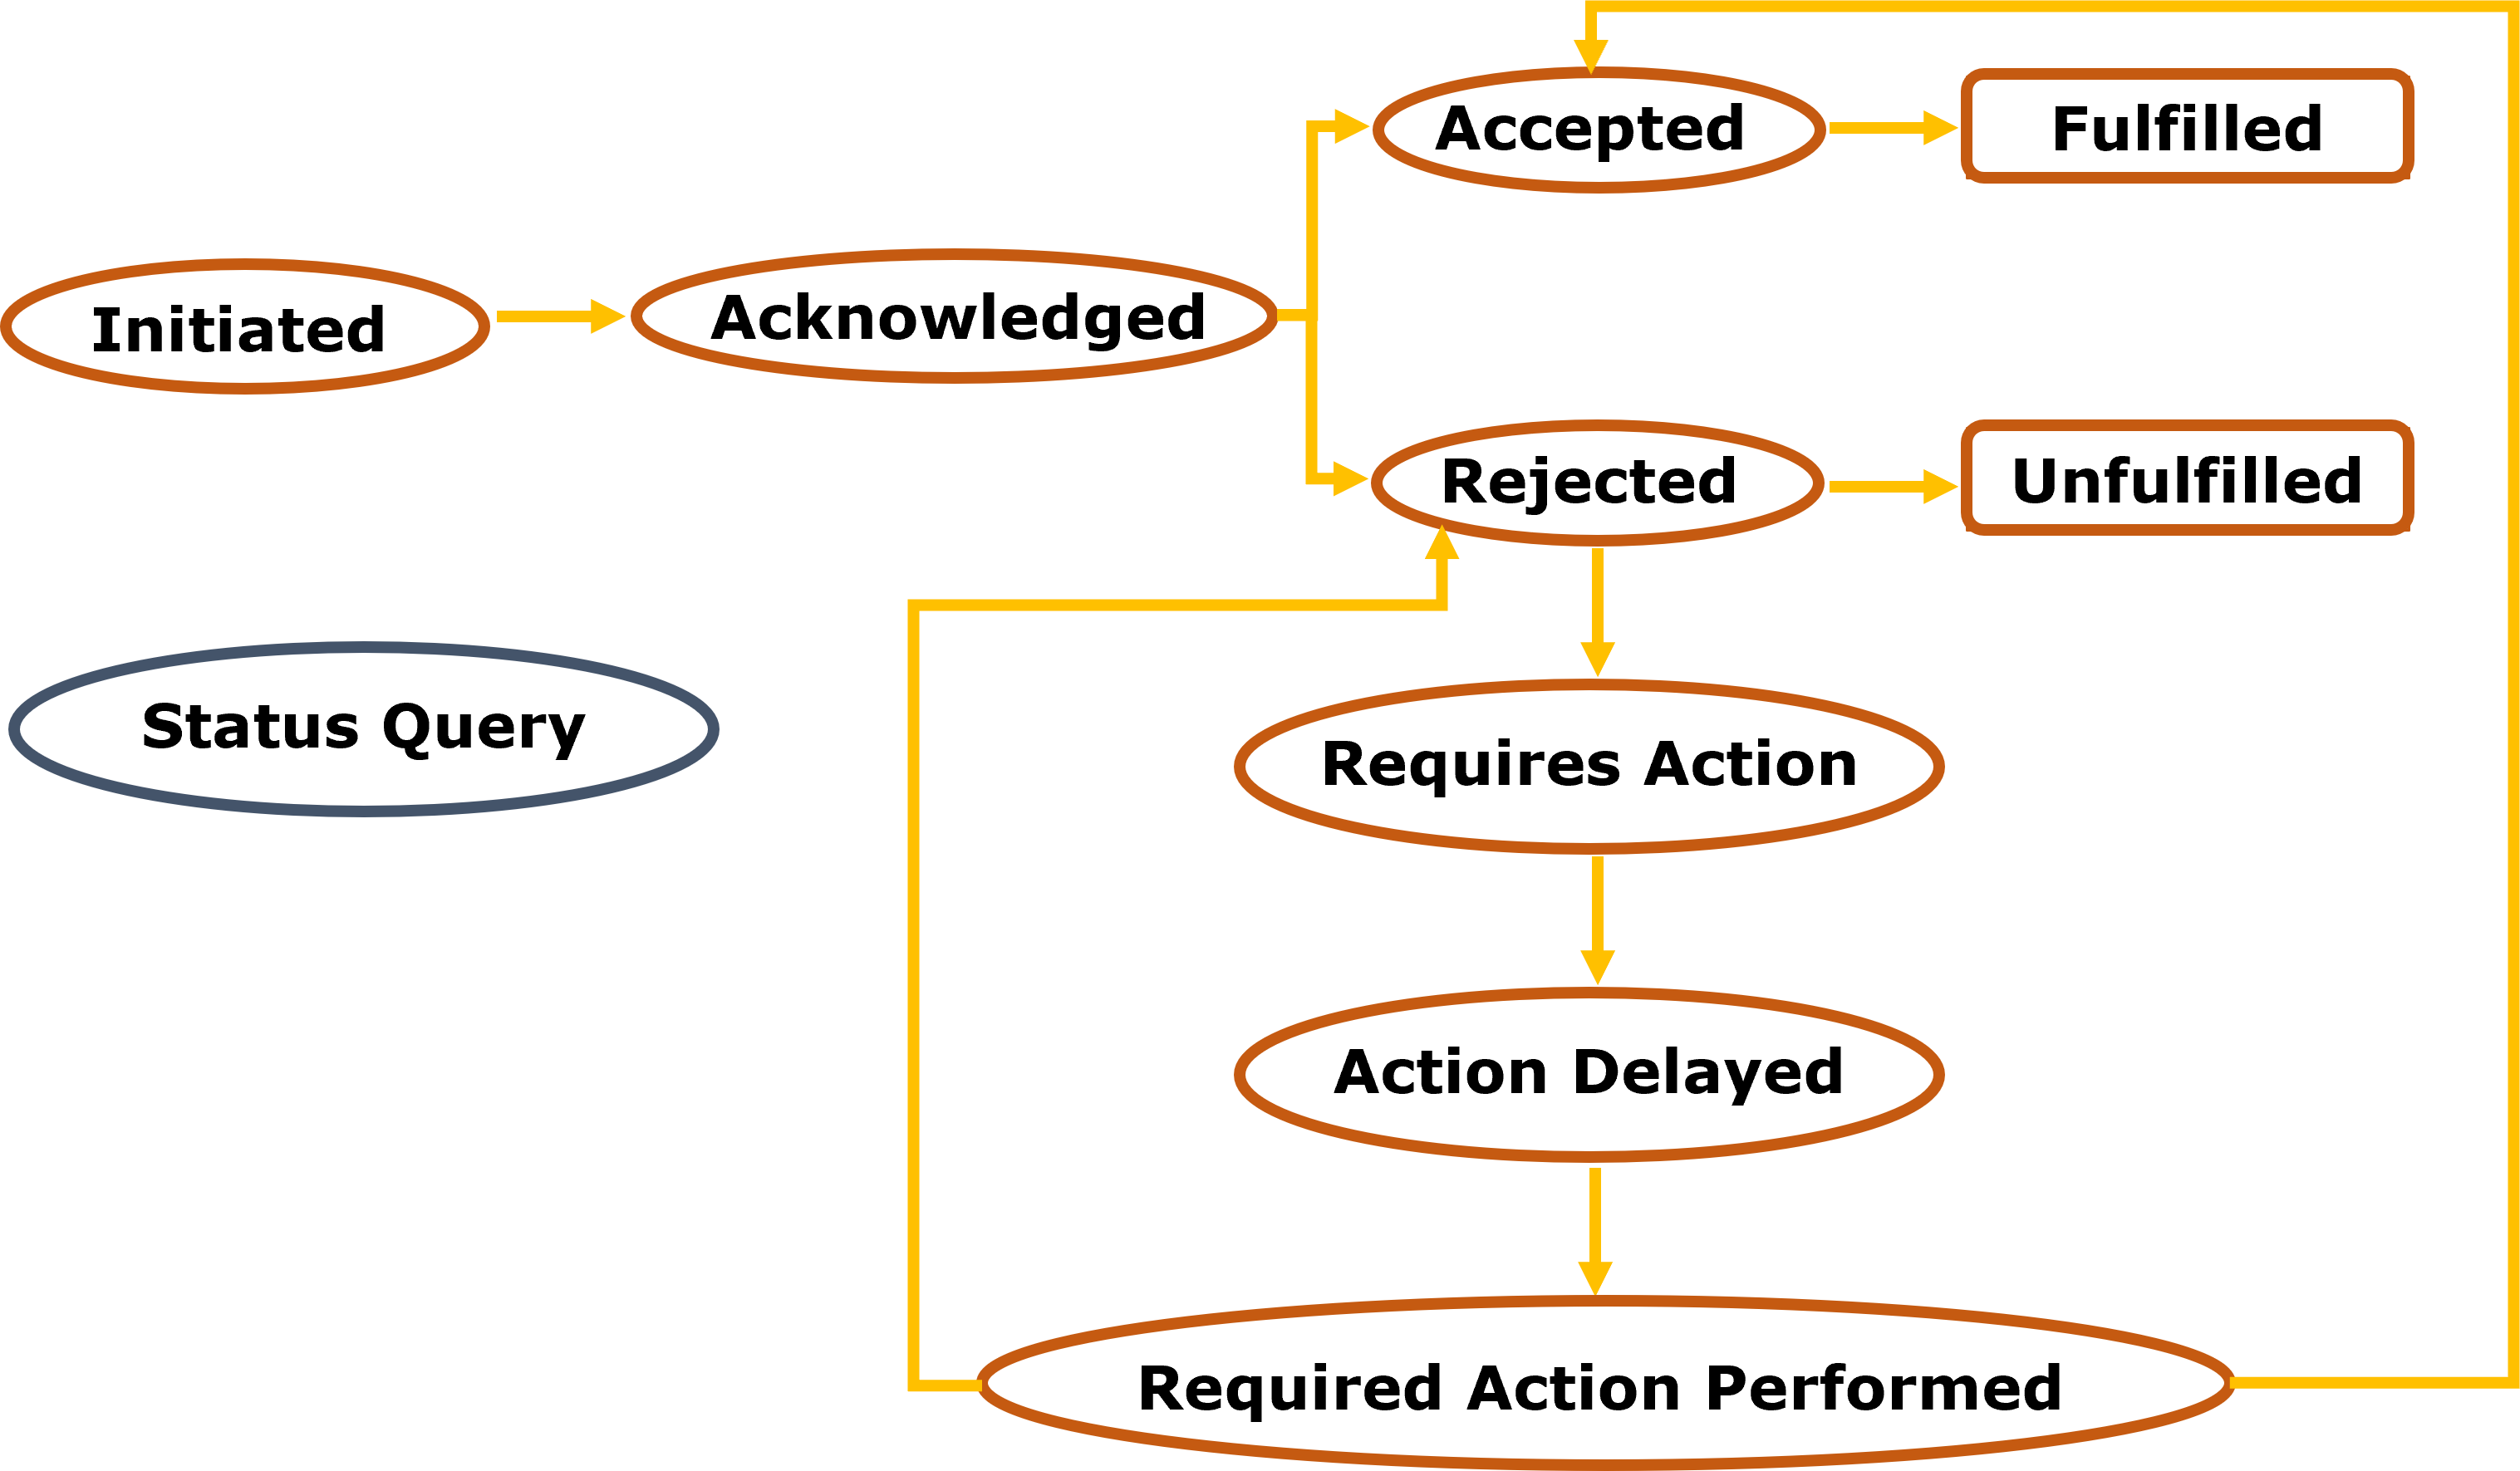
\includegraphics[width=0.8\linewidth]{figures/chapter-4/request-status.png}
    \caption{DPV's concepts to model the status of a request.}
    \label{fig:request_status}
\end{figure}

Listing~\ref{list:request_acknowledgment} illustrates a record of the right exercising activities related to a GDPR right of access request and acknowledgement of said request.
The activity associated with the start of the request has the status \texttt{dpv:RequestInitiated}, the data subject is identified using the \texttt{dpv:hasDataSubject} and the recipient of the request, a data controller, using the \texttt{dpv:hasRecipientDataController}.
Furthermore, a personal data handling instance can be used to express what personal data needs to be processed for the fulfilment of the right and DPV's \texttt{hasScope} to specify the scope of the request, e.g., the data subject only wants to access data processed for service provision purposes or only data processed during 2022.
Following the start of the request, the controller acknowledges the request, a right exercising activity which has \texttt{dpv:RequestAcknowledged} status and the recipient is the data subject that initiated the request.

\begin{listing}[htp]
\caption{Record of GDPR right of access request and acknowledgement activities.}
\label{list:request_acknowledgment}
\begin{minted}{turtle}
ex:DataSubject a dpv:DataSubject .
ex:DataSubjectUsername a dpv-pd:AccountIdentifier ;
    dpv:hasDataSubject ex:DataSubject .

ex:SARequest a dpv:RightExerciseActivity, prov:Activity ;
    dcterms:description "Data Subject makes a GDPR right of access request" ;
    dpv:hasRight dpv-gdpr:A15 ;
    dpv:isExercisedAt ex:RightExercisePoint ;
    prov:wasAssociatedWith ex:DataSubject ;
    dpv:hasDataSubject ex:DataSubject ;
    dpv:hasRecipientDataController ex:DataController ;
    dcterms:date "2023-11-02T11:08:05"^^xsd:dateTime ;
    dpv:hasStatus dpv:RequestInitiated ;
    dpv:hasPersonalDataHandling [
        a dpv:PersonalDataHandling ;
        dpv:hasPurpose dpv:IdentityVerification ;
        dpv:hasPersonalData ex:DataSubjectUsername ;
        dpv:hasProcessing dpv:Collect, dpv:Store ] ;
    dpv:hasScope [
        dpv:hasPurpose dpv:ServiceProvision ;
        dpv:hasDuration [
            time:hasBeginning "2022-01-01T00:00:00"^^xsd:dateTime ;
            time:hasEnd "2022-12-31T23:59:59"^^xsd:dateTime ] ] .

ex:SARAcknowledged a dpv:RightExerciseActivity, prov:Activity ;
    dcterms:description "Data controller acknowledges the request" ;
    dcterms:date "2023-11-02T15:55:10"^^xsd:dateTime ;
    prov:wasAssociatedWith ex:DataController ;
    dpv:hasRecipient ex:DataSubjectUsername ;
    dpv:hasStatus dpv:RequestAcknowledged ;
    dpv:isAfter ex:SARequest .
\end{minted}
\end{listing}

Listing~\ref{list:further_action} illustrates the follow-up to Listing~\ref{list:request_acknowledgment} -- the request was rejected due to an \texttt{IdentityVerificationFailure} and as such the data controller requires further information from the data subject to be able to proceed with the request.
Such right exercise activity is identified with the \texttt{dpv:RequestRequiresAction} status and contains a personal data handling activity instance expressing the information that the data subject needs to provide for the right exercise to continue.
Afterwards, a right exercise activity associated with the data subject and with a \texttt{dpv:RequestRequiredActionPerformed} status is recorded with the information that the data subject provided.

\begin{listing}[htp]
\caption{Record of data controller requesting further information to fulfil the data subject's SAR and of the data subject providing the controller with said information.}
\label{list:further_action}
\begin{minted}{turtle}
ex:SARRejected a dpv:RightExerciseActivity, prov:Activity;
    dcterms:description "Data controller rejects the request" ;
    dcterms:date "2023-11-02T15:57:31"^^xsd:dateTime ;
    prov:wasAssociatedWith ex:DataController ;
    dpv:hasRecipient ex:DataSubjectUsername ;
    dpv:hasStatus dpv:RequestRejected ;
    dpv:hasJustification rights:IdentityVerificationFailure ;
    dpv:isAfter ex:SARAcknowledged .

ex:SARRequiresAction a dpv:RightExerciseActivity, prov:Activity ;
    dcterms:description "Data controller requires further actions" ;
    dcterms:date "2023-11-02T16:09:21"^^xsd:dateTime ;
    prov:wasAssociatedWith ex:DataController ;
    dpv:hasRecipient ex:DataSubjectUsername ;
    dpv:hasStatus dpv:RequestRequiresAction ;
    dpv:hasJustification rights:IdentityVerificationFailure ;
    dpv:hasPersonalDataHandling [
        dpv:hasPersonalData dpv-pd:OfficialID ;
        dpv:hasProcessing dpv:MakeAvailable ;
        dpv:hasPurpose dpv:IdentityVerification ;
        dpv:hasRecipientDataController ex:DataController ;
        dpv:isImplementedByEntity ex:DataSubjectUsername ] ;
    dpv:isAfter ex:SARRejected .

ex:DataSubjectOfficialID a dpv-pd:OfficialID ;
    dpv:hasDataSubject ex:DataSubject .

ex:SARActionPerformed a dpv:RightExerciseActivity, prov:Activity ;
    dcterms:description "Data Subject provides required information" ;
    dcterms:date "2023-11-02T17:20:42"^^xsd:dateTime ;
    prov:wasAssociatedWith ex:DataSubject ;
    dpv:hasStatus dpv:RequestRequiredActionPerformed ;
    dpv:hasPersonalDataHandling [
        dpv:hasPersonalData ex:DataSubjectOfficialID ;
        dpv:hasProcessing dpv:MakeAvailable ;
        dpv:hasPurpose dpv:IdentityVerification ;
        dpv:hasRecipientDataController ex:DataController ;
        dpv:isImplementedByEntity ex:DataSubjectUsername ] ;
    dpv:isAfter ex:SARRequiresAction .
\end{minted}
\end{listing}

Listing~\ref{list:sar_notice} illustrates the follow-up to Listing~\ref{list:further_action} -- the request was accepted and fulfilled by the data controller and as such the data controller provides the data subject with a notice of the fulfilment of GDPR's Art.15, modelled as a \texttt{dpv-gdpr:SARNotice}, and a copy of the data whose access was requested, modelled as a \texttt{dcat:Dataset}.
Beyond temporal information and providing the location of the notice, a personal data handling instance can be used to provide additional information to the data subject -- in the case of this SAR notice, the data subject is also notified of the type of personal data being processed, the purpose for the processing, the time period when the data was processed and the additional data subject rights that can be exercised.

\begin{listing}[htp]
\caption{Record of the acceptance and fulfilment of the request and respective \texttt{SARNotice}.}
\label{list:sar_notice}
\begin{minted}{turtle}
ex:SARAccepted a dpv:RightExerciseActivity, prov:Activity ;
    dcterms:description "Request accepted by data controller towards fulfilment" ;
    dcterms:date "2023-11-03T08:15:04"^^xsd:dateTime ;
    prov:wasAssociatedWith ex:DataController ;
    dpv:hasRecipient ex:DataSubjectUsername ;
    dpv:hasStatus dpv:RequestAccepted ;
    dpv:isAfter ex:SARActionPerformed .

ex:SARFulfilled a dpv:RightExerciseActivity, prov:Activity ;
    dcterms:description "Request fulfilled by data controller" ;
    dcterms:date "2023-11-03T08:37:25"^^xsd:dateTime ;
    prov:wasAssociatedWith ex:DataController ;
    dpv:hasRecipient ex:DataSubjectUsername ;
    dpv:hasStatus dpv:RequestFulfilled ;
    prov:generated ex:DataCopy, ex:SARNotice_Username ;
    dpv:isAfter ex:SARAccepted .

ex:SARNotice_Username a dpv-gdpr:SARNotice ;
    dcterms:date "2023-11-03T08:31:51"^^xsd:dateTime ;
    foaf:page <https://example.com/DataController/SARNotice_Username> ;
    dpv:hasPersonalDataHandling [
        a dpv:PersonalDataHandling ;
        dpv:hasPersonalData dpv-pd:EmailAddress ;
        dpv:hasPurpose dpv:ServiceProvision ;
        dpv:hasDuration [
            time:hasBeginning "2022-01-01T00:00:00"^^xsd:dateTime ;
            time:hasEnd "2022-12-31T23:59:59"^^xsd:dateTime ] ;
        dpv:hasRight dpv-gdpr:A16, dpv-gdpr:A17, dpv-gdpr:A18, dpv-gdpr:A21, dpv-gdpr:A77 ] .

ex:DataCopy a dcat:Dataset ;
    dcterms:format <https://www.iana.org/assignments/media-types/text/csv> ;
    dcterms:accessRights access-right:c_16ec ; # restricted access
    dcterms:issued "2023-11-03T08:35:42"^^xsd:dateTime ;
    dcterms:valid "2023-12-03T08:35:42"^^xsd:dateTime ;
    dcat:landingPage <https://example.com/Username/SAR_DataCopy> .
\end{minted}
\end{listing}

Moreover, DCAT \citep{albertoni_data_2020} can be used to model resources beyond notices, for instance, a copy of the personal data, in the case of a right of access request according to the GDPR, as in Listing~\ref{list:sar_notice}.
Information regarding the format, validity and dataset provision/download location can be attached to the dataset representation using the \texttt{dcterms:format}, \texttt{dcterms:valid} and \texttt{dcat:landingPage} properties, respectively.
Additionally, DCAT -- and also the Data on the Web Best Practices Recommendation \citep{loscio_data_2017} -- promotes the usage of ODRL to express license and rights statements, by linking the dataset with an ODRL policy using the \texttt{odrl:hasPolicy} property, or the usage of DCMI Metadata Terms' \texttt{license}, \texttt{accessRights} or \texttt{rights} properties to link datasets with licenses, access rights statements or other types of rights statements, e.g., copyrights, respectively.
In the case of using the latter, controlled vocabularies such as COAR's Access Rights vocabulary \citep{apollaro_controlled_2022}, used in Listing~\ref{list:sar_notice} to restrict access only to the data subject, or the Named Authority List of Access rights from the \cite{publications_office_of_the_european_union_named_2023} can be used to express `high-level' access control statements, e.g., embargoed, restricted or open access.

In this Section, the GDPR's Right of Access is used as an example to showcase how to model notices and right exercising activities using DPV, DCMI Metadata Terms, PROV-O and DCAT.
However, a similar pattern can be followed by data controllers to fulfil the other rights as in most cases the only substantial change would be the notice concept that needs to be used for a particular right instance, e.g., \texttt{dpv-gdpr:DirectDataCollectionNotice} for the right fulfilment notice related to GDPR's Article 13, \texttt{dpv-gdpr:IndirectDataCollectionNotice} for the right fulfilment notice related to GDPR's Article 14 or \texttt{dpv-gdpr:RightsRecipientsNotice} for the right fulfilment notice related to GDPR's Article 19.
Moreover, some GDPR rights, such as the right to erasure in Article 17 and the right to restriction of processing in Article 18, also require the data subject to provide a justification for their request to be fulfilled by the data controller.
A collection of justifications for the fulfilment of data subject rights, extracted from the GDPR and illustrated in Table~\ref{tab:fulfil_justifications}, was also modelled (as subclasses of a high-level \texttt{RightFulfilmentJustification} concept). % and is already approved to be integrated into DPV-GDPR's outputs.

\begin{table}
    \centering
    \caption[Justifications for the fulfilment of GDPR's data subject rights]{Justifications for the fulfilment of GDPR's data subject rights. PD is used in the terms to shorten `Personal Data'.}
    \label{tab:fulfil_justifications}
    \resizebox{\textwidth}{!}{%
    \begin{tabular}{c|p{8.5cm}|c}
        \textbf{Term} & \textbf{Label} & \multicolumn{1}{c}{\begin{tabular}[c]{@{}c@{}} \textbf{GDPR} \\ \textbf{Article(s)} \end{tabular}} \\
        \hline\hline
        \texttt{RightFulfilmentJustification} & Justifications for the fulfilment of a right & \\
        \hline\hline
        \texttt{ProcessingNotNecessary} & \multicolumn{1}{l|}{\begin{tabular}[l]{@{}l@{}} Processing no longer necessary for the \\specified purposes \end{tabular}} & 17.1(a) \\
        \hline
        \texttt{DataSubjectWithdrewConsent} & \multicolumn{1}{l|}{\begin{tabular}[l]{@{}l@{}} Data subject withdrew consent and there is \\no other legal ground for the processing \end{tabular}} & 17.1(b) \\
        \hline
        \texttt{DataSubjectObjectedToProcessing} & Data subject objected to the processing & 17.1(c), 18.1(d) \\
        \hline
        \texttt{PDUnlawfullyProcessed} & Personal data unlawfully processed & 17.1(d), 18.1(b) \\
        \hline
        \texttt{ComplianceWithLegalObligation} & Compliance with a legal obligation & 17.1(e) \\
        \hline
        \texttt{PDForInformationSocietyServices} & \multicolumn{1}{l|}{\begin{tabular}[l]{@{}l@{}} Personal data collected in relation to the offer \\of information society services \end{tabular}} & 17.1(f) \\
        \hline
        \texttt{AccuracyOfPDContested} & \multicolumn{1}{l|}{\begin{tabular}[l]{@{}l@{}} Accuracy of personal data contested by the \\data subject \end{tabular}} & 18.1(a) \\
        \hline
        \texttt{LegalClaims} & \multicolumn{1}{l|}{\begin{tabular}[l]{@{}l@{}} Data subject requires the personal data for the \\establishment, exercise or defence of legal claims \end{tabular}} & 18.1(c) \\
    \end{tabular}}
\end{table}

% TODO: add \subsection{Vocabulary publication and maintenance}\label{sec:plasma_publication} later on